%cSpell:ignore Erol,Sezgin,fancyhdr, hheadheighti,hheadsepi,hfootheighti,graphicx, hfootskipi, Gavrilita, Mihail, AMOO, totalheight, keepaspectratio,UML's, kata, codewars, OOAD, COFFE,ERLANG,caml, kotlin,haskel, ruby, superclass, 
\documentclass[12pt]{article}
%\usepackage[english]{babel}
%actually it works without this package//// cuz it is in english by default... it might be useful //// but not here
% \usepackage{natbib}
% \usepackage{biblatex}

% \usepackage[backend=biber]{biblatex}

%\usepackage{url}
%idk what for it is here, it is not what it seems to be, fuck it
%%\usepackage[document]{ragged2e} 
%%to justify
% i dont use it anymore
\usepackage[utf8]{inputenc}
%%%\usepackage{amsmath}
%%useless for this report... it's for math stuff
\usepackage{graphicx}
%This package enables the user to the importation of graphics into a .tex file and, apart from the usual sizing and rotational facilities, also enables the user to crop or trim an image as desired (e.g., to get rid of surrounding blank margins). The graphicx package is useful if you need to use only a part of a complete image. 
\graphicspath{{images/}}
%% includes pics inside image folder
\usepackage{parskip}
%%this shit . In the document body, don't use \parskip but a blank line to separate paragraphs.there's normally no need to add manual line breaks (\\) in the text.

\usepackage{vmargin}
%%LaTeX package which introduces paper sizes and provides macros for setting document margins. 
\usepackage{enumerate} 
%enumeration of elements  
\usepackage{caption}
%%this is for figures
\usepackage{float}
%% to position exactly the figure 
\usepackage{fancyhdr}
%%To customize the footer and header in your document first import the package fancyhdr with 
% \addbibresource{lab4.bib}
% \bibliography{my_bibliography.bib} 
\PassOptionsToPackage{hyphens}{url}\usepackage{hyperref}
\hypersetup{
    colorlinks=true,
    linkcolor=blue,
    filecolor=magenta,      
    urlcolor=cyan,
}

\renewcommand{\theenumii}{\arabic{enumii}}
\setmarginsrb{3 cm}{2.5 cm}{3 cm}{2.5 cm}{1 cm}{1.5 cm}{1 cm}{1.5 cm}
%%\setmarginsrb{hleftmargini}{htopmargini}{hrightmargini}{hbottommargini}% {hheadheighti}{hheadsepi}{hfootheighti}{hfootskipi
\title{DB Laboratory 3}								
\author{Sezgin E}							
\makeatletter
%%The \makeatletter command temporarily defines »@« as a normal character to enable changes to internal LaTeX macros outside packages (STY) or classes (CLS).
\let\thetitle\@title
%%\let allows you to copy the content of a command into a new command.
\let\theauthor\@author
%%Thus \let\foo\bar defines \foo to have the value that \bar had at the point of definition.
\makeatother
% With \makeatother this process is reversed and the »@« is set to its original character category (other). The »@« is used to protect the internal LaTeX macros. Hence you should be very careful when using these two commands.
\pagestyle{fancy}
%%After that, the "fancy" style is set by \pagestyle{fancy}
\fancyhf{}
%%The command \fancyhf{} clears the header and footer, otherwise the elements of the default "plain" page style will appear. 
\rhead{\theauthor}
%%Prints the text included inside the braces on the right side of the header. 
\lhead{\thetitle}
%%Prints the text set inside the braces on the left side of the header.
\cfoot{\thepage}
%%\cfoot{Page \thepage}  Prints the word "Page" and next the page number which is automatically set by \thepage on the center of the footer. 
        
\begin{document}
        
        %%%%%%%%%%%%%%%%%%%%%%%%%%%%%%%%%%%%%%%%%%%%%%%%%%%%%%%%%%%%%%%%%%%%
        
        \begin{titlepage}
                \centering
                \vspace*{0.5 cm}
                
\includegraphics[scale = 0.11]{LOGO_UTM.jpg}\\[1.0 cm]	% University Logo
                %% Importing a graphic is done by using the command \includegraphics[key1=...,key2=...,etc.]{filename} Optional parameters—called “keys”—enable the figure to be resized, rotated, cropped, trimmed, etc. These keys and their functions are listed below. 
                %• scale = number — a magnification factor 
                %• width = length — the width to which the figure should be scaled1
                %• height = length — the height to which the figure should be scaled2 
                %• totalheight = length — height plus depth of figure (to be used if figure is rotated) 
                %• keepaspectratio = true/false — maintains the height/width ratio 
                %• angle = number — angle (in degrees) by which the figure is to be rotated counterclockwise 
                %• origin = location3 — the point about which rotation is to occur %• draft = true/false — prevents figure from being imported, but created a named box with the dimensions of the figure (this option is used to speed up processing) 
                %• clip = true/false — excludes whatever is outside the bounding box 
                \textsc{\LARGE Technical University of Moldova}\\[2.0 cm]%%\textsc{example text} will display the example text as small caps. All of the letters will be capitalized/uppercase, but they are going to be similar in size to a lowercase letter.	
                % University Name
                \textsc{\Large 24.09.2018}\\[0.5 cm]		% Course Code

                \rule{\linewidth}{0.2 mm} \\[0.4 cm]
                %%The \rule command in normal use produces a simple black box: \rule[raise]{width}{thickness} This is useful for drawing vertical and horizontal lines.

                { \huge \bfseries \thetitle}\\
                %%Anyway, the \bfseries bold the rest of my document, even though I'm using curly braces.
                \rule{\linewidth}{0.2 mm} \\[1.5 cm]
                
                \begin{minipage}{0.4\textwidth}
                        \begin{flushleft} \large
                                \emph{Submitted To:}\\
                                Maria Cojanu\\
                %%If you want to emphasize a word or some text, use \emph. Don't just make the text italic or bold. If needed, you may change the behavior of \emph whenever you wish in the preamble and the whole document will be adjusted accordingly.
                Asst. Univ.\\
                Computer Science Department\\
                            \end{flushleft}
                            \end{minipage}~
                            \begin{minipage}{0.4\textwidth}
                
                            \begin{flushright} \large
                            \emph{Submitted By :} \\
                            Sezgin Erol\\
                
                Group FAF-161\\
                Semester 1\\
                    \end{flushright}
                
                \end{minipage}\\[2 cm]
                
                \vfill Chisinau 2018\\  
        \end{titlepage}
        
        %%%%%%%%%%%%%%%%%%%%%%%%%%%%%%%%%%%%%%%%%%%%%%%%%%%%%%%%%%%%%%%%%%%%
        \pagebreak
        %\tableofcontents
        \subsection*{ General purpose:}
        \subsubsection*{ Learn about Creating Table of DataBase}
        
        \subsection*{Tasks:}
        \begin{itemize}
                \item Answer Questions at the end of Chapter 4;
                \item Solve ex. 1, 2 at the end of Chapter 4;
                \item Create a database which name is "Universitate";
                \begin{itemize}
                        \item Grupe;
                        \item Discipline;
                \end{itemize}
                \item Create the following tables on your database;
        \end{itemize}
        \subsection*{Answers to Questions:}
        \begin{enumerate}
                \item In SQL Server any column in a database table must have at least those properties specified:
                \begin{itemize}
                        
                        \item Name - the name of the selected column.
                        \item Data Type - the data type for the selected column.
                        \item Allow Nulls - indicates whether this column allows nulls.

                \end{itemize}
                \item Some of the data types used in SQL Server;
                \begin{itemize}                   
                        \item Exact numerics (bigint, int, smallint, bit, decimal, etc.)
                        \item Approximate numerics (float, real)
                        \item Character Strings (char, varchar, text)
                        \item Date and time (date, datetime, smalldatetime, etc.)
                        \item Binary strings (binary, varbinary, image)
                        \item Other data types (cursor, hierarchyid, rowversion, etc.)
                        \item Unicode character strings (nchar, nvarchar, ntext)
                \end{itemize}
                \item Integrity constraints are used to ensure accuracy and consistency of data in a relational database. SQL Server uses following constraints
                \begin{itemize}                       
                        \item Not NULL - disallows the entrance of NULL values into a column
                        \item Unique - value in that column for every row of data in the table must have a unique value.
                        \item Primary Key - identifies one or more columns in a table that make a row of data unique.
                        Foreign Key - references a primary key in the parent table.
                        \item Check - Check (CHK) constraints can be utilized to check the validity of data entered into particular table columns.
                \end{itemize}
                \item You cannot delete a column that has a CHECK constraint without deleting the constraint first. Also, it is not possible to delete a column that has PRIMARY KEY or FOREIGN KEY constraints or other dependencies except when using the Table Designer. When using Object Explorer or Transact-SQL, you must first remove all dependencies on the column.
                \item Modifying the data type of a column that already contains data can result in the permanent loss of data when the existing data is converted to the new type. In addition, code and applications that depend on the modified column may fail. These include queries, views, stored procedures, user-defined functions, and client applications. Note that these failures will cascade. For example, a stored procedure that calls a user-defined function that depends on the modified column may fail.
        \end{enumerate}


        \subsection*{Task Realization:}
        \begin{enumerate}
                \item  Which number can be put in a column with type DECIMAL(4, 1)?
                \begin{itemize}
                        \item 116,2 is answer because it exactly 4 digits with 1 digits after comma.
        
                \end{itemize}
                \item Consider Col1 is INT and Col2 is DECIMAL(2, 1). What type Col3 should be to contain the result of Col1 * Col2?
                \begin{figure}[H]
                        \centering
                        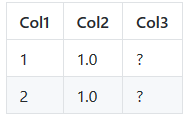
\includegraphics[width=.35\textwidth]{task2.png}
                        \caption{Creating The table "Grupe"}
                \end{figure}
                \vspace{0.5 cm}

                In order to save the result of multiplication Col3 must have DECIMAL(2, 1) as type, since DECIMAL has higher precedence than INT
        \end{enumerate}
       

        
        In figure 2 I created the table "Grupe". And i set the data types for each row.
        \begin{figure}[H]
                \centering
                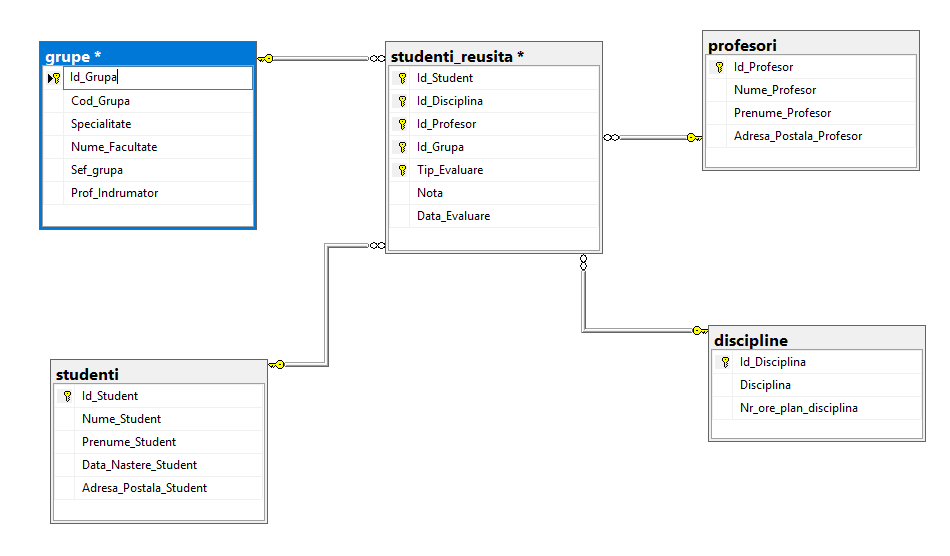
\includegraphics[width=.95\textwidth]{img1.png}
                \caption{Creating The table "Grupe"}
        \end{figure}
        \vspace{0.5 cm}
        In figure 3 I created the second table: "Discipline". And also i set the data types for each row. 
        
        \begin{figure}[H]
                \centering
                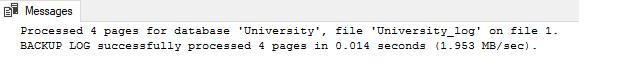
\includegraphics[width=.95\textwidth]{img2.png}
                \caption{Creating The table "Discipline" }
        \end{figure}
        \vspace{0.5 cm}

        
        \begin{figure}[H]
                \centering
                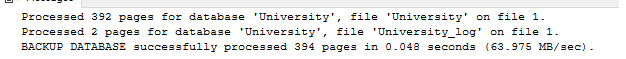
\includegraphics[width=.95\textwidth]{img3.png}
                \caption{fulfilling The table "Discipline"}
        \end{figure}
        \vspace{0.5 cm}

        
        \begin{figure}[H]
                \centering
                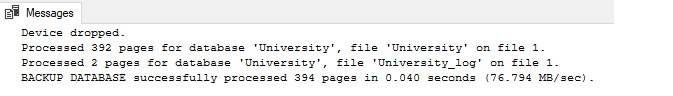
\includegraphics[width=.95\textwidth]{img4.png}
                \caption{fulfilling The table "Grupe"}
        \end{figure}
        \vspace{0.5 cm}

        \newpage 
        \subsection*{Conclusion}
        During This lab work i find out how to create tables, name the table rows, set primary keys, and set the data types of columns in that table. Also i learned how to fulfil the table with data, make some changes in the structure of that tables, etc.
        \cite{SQLServerManagementStudio}
        

 
\medskip
 
\begin{thebibliography}{9}
\bibitem{SQLServerManagementStudio} 
SQL Server Management Studio 2017, Tutorials for Lab 3

\end{thebibliography}
                
\end{document}